\section{Generality}
\label{sec:generality}

% as depicted in Figure~\ref{fig:workflow}
Although this paper examines the methodology on GPU Kepler architecture and shows its performance optimizations for SGEMM, we claim that the developed toolchain can be easily extended to other NVIDIA GPUs and the explored optimization strategies are applicable to other floating-point computation-intensive applications.

{\em {\bf Generality of the toolchain}}: For a particular GPU architecture, users only need to regenerate disassembly codes from the PTX samples and microbenchmarks with CUDA binary utilities, and then feed them to the ISA encoding solver.
The opcode, modifier and operand solvers, are portable among GPU architectures. 
We have validated the solver functionalities on Fermi, Kepler, and Maxwell GPUs. 
A corresponding assembler can be obtained by modifying the instruction grammar definition decoded by the solver, which could be automatically done with an assembler template provided by Gray~\cite{baldassin2005extending}.

{\em {\bf Generality of optimizations}}: The optimization strategies include
FFMA dual-issue, register allocation, memory load/store width, and instruction
scheduling. The latter three strategies are applicable to other GPU
architectures by leveraging the benchmarks to detect effective parameters. 
Only the first one is specific to Kepler architecture. 


Note that the low-level optimizations are more microarchitectural specific than application specific. 
Usually, a float computation-intensive application can be optimized using
blocking or tiling to improve the ratio of computation to memory access and hide memory latency. 
Only if register blocking is used, multiple float computation instructions will be reside in a single loop iteration, then register allocation and dual issue optimization can refer SGEMM optimizations to improve float computation throughput. 
With the support of a assemble language, our scheduling optimization is totally derived from instruction dependency and latency, which is not specific to SGEMM. 
Applications with contiguous memory access pattern can use {\tt LDG.128} to reduce the number of memory instructions.
%\jli{deleted, because this is specific to Kelper: ``{\tt LDS.64} achieves best bandwidth on Kepler due to 8 bytes per shared memory bank.'' }
%We also vertified these two memory instruction achieve best for convolution algorithm.
As the previous investigations of GEMM optimization on CPUs have inspired
general performance tuning and compiler optimizations~\cite{lam1991cache}, this work attempts to stimulate more meticulous performance tuning on GPUs.  
%Although we use a exhaust search method to search the optimal scheduling, we
%argue that the idea may be applicable to general optimizations
%because small piece of code often occupy most of the
%execution time in a lot of scientific and engineering applications.
%As an alternative way, auto-tuning techniques~\cite{} 
%can be taken to find a better scheduling order. 
%For another floating-point intensive algorithm like convolution in deep learning applications, the FFMA throughput can be improved by eliminating register bank conflicts and activating dual issue. Then non-FFMA instructions are carefully scheduled without affecting the FFMA throughput. 

{\em {\bf Convolutional Algorithm Performance}}:
%\jli{give one more sentence for convolutional algorithms}
%We optimize a convolution algorithm at assembly level using the method described in Section~\ref{sec:optimization}.
%Our convolution algorithm uses $128\times128$ shared memory blocking and $8\times8$ register blocking. 
%Three popular convolutional neural networks, Alexnet~\cite{krizhevsky2012imagenet}, Vgg~\cite{simonyan2014very} and Overfeat~\cite{sermanet2013overfeat}, are tested 
%We refer interested readers to these papers for detailed network configurations.
% The configuration of each convolutional layer can be found in corresponding papers.
Our convolution algorithm implementation uses $128\times128$ shared memory blocking and
$8\times8$ register blocking. We optimize it at assembly-level by using the method describe in section~\ref{sec:optimization}.
%The configuration of each layer can be found 
We benchmark three popular convolutional neural network:
Alexnet~\cite{krizhevsky2012imagenet}, Vgg~\cite{simonyan2014very} and
Overfeat~\cite{sermanet2013overfeat}.  The configuration of each convolutional
layer can be found in corresponding papers.
Figure~\ref{fig:conv} presents the performance of our optimized convolution and cuDNN by comparing the average performance of all the convolutional layers in a neural network. %The maximum convolution performance is 2653 Gflop/s.
Our optimized convolution implementations are 39\%, 46\% and 62\% higher than cuDNN V4.0 for the three CNN configurations respectively on Tesla K20m.

\begin{figure}[htbp]
\begin{center}
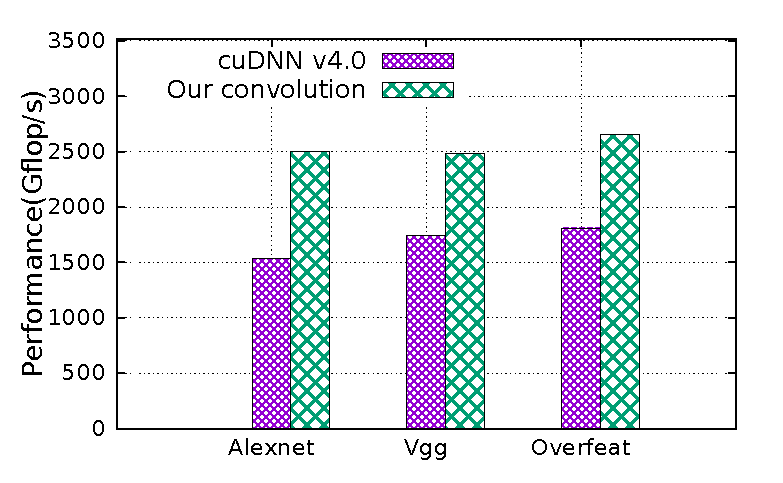
\includegraphics[scale=0.5]{cudnn}
    \caption{Performance comparison of cuDNN and our optimized convolution on GPU Tesla K20m (batch size is 128).}
\label{fig:conv}
\end{center}
\end{figure}
